%\nonstopmode
\hbadness=100000
\documentclass[a4paper, 12pt]{article}
\usepackage{amsmath,amsfonts,caption,float,geometry,graphicx,mathtools,pythonhighlight,textcomp,url,verbatim,subcaption,tabularx, longtable, ulem, hyperref,extarrows,glossaries} %,parskip
\geometry{ a4paper, total={170mm,257mm}, left=20mm, top=20mm}
\newcommand{\matr}[1]{\underline{\underline{\textbf{#1}}}}
\newcommand{\ve}[1]{\boldsymbol{#1}}
\DeclareMathOperator*{\argmax}{arg\,max}
\DeclareMathOperator*{\argmin}{arg\,min}
\newcommand{\pythoncode}[2]{
\begin{adjustwidth}{-1.3cm}{-1.3cm}
\texttt{#1}
\inputpython{#2}{1}{1500}
\end{adjustwidth}
}
\usepackage[toc, page]{appendix}
% \usepackage[dvipsnames]{xcolor}
% \definecolor{subr}{rgb}{0.8, 0.33, 0.0}
% \definecolor{func}{rgb}{0.76, 0.6, 0.42}
\begin{document}
    
\centering
% \includegraphics[width=8cm]{CoverPage/UoBlogo.pdf}
% \hrule
% \bigbreak
% \textbf{F}usion Neutron \textbf{Acti}vation Spectra \textbf{U}nfolding by \textbf{N}eural \textbf{N}etworks \\
% (FACTIUNN)                                      \\
% \hrule
% \bigbreak
% \begin{minipage}[b]{0.4\textwidth}
%     \includegraphics[height=2cm]{CoverPage/CCFElogo.jpeg}
%   \end{minipage}
%   \hfill
%   \begin{minipage}[b]{0.4\textwidth}
%     \includegraphics[height=3cm]{CoverPage/UKAEAlogo.jpeg}
% \end{minipage}
    
\begin{table}[!h]
\centering
\begin{tabular}{rl}
author:&Ocean Wong          \\
       &(Hoi Yeung Wong)    \\
supervisor:&Chantal Nobs    \\
           &Robin Smith     \\
date:  &2019-11-14 14:26:00 \\
Organization:  &Culham Centre for Fusion Energy
\end{tabular}
\end{table}
\hrule
\bigbreak
\abstract
A short document to explain how to choose the most effective set of activation foils for neutron spectrum unfolding.
(This document will be expanded upon later, i.e. in the coming month)    
% \emph{Keywords:} Effectivenss matrix
% \hline
% \twocolumn
% \pagebreak
% \tableofcontents
% \listoffigures
% \pagebreak
\hrule
\vspace{1cm}
\chapter{}
Notations:

$\ve{V}$ectors (column vectors), \matr{M}atrices, $\cdot$ dot product.

$\sigma_{\text{no subscript}}(\text{a quantity})$= uncertainy of the quantity; $\sigma_{\text{with subscript(s)}}$= microscopic cross-section

% \textit{Note that in this document, $\sigma$ is used for both microscopic cross-section and standard deviation. When it is appended by subscript(s), (e.g. $\sigma_i$) it is used to denote microscopic cross-section; otherwise it must be \emph{immediately} followed by a bracketed quantity (e.g. $\sigma(N)$) which denotes the standard deviation of the bracketed quantity (e.g. $N$).}
%Need to insert graph of illustration of unfolding process

\begin{equation}
    \begin{matrix}
        (\ve{\phi_{true}}) & \rotatebox[origin=c]{-20}{$\xLongrightarrow{\matr{R}}$}\\
        && \ve{Z} & \xLongrightarrow[\text{and irradiation period}]{\text{integrate over volume}} & \ve{N_\infty} & \xLongrightarrow[\text{transit}]{\text{decay during}} & \ve{N_0} & \xLongrightarrow{detection} & \ve{C_0}\\
        \ve{\phi_{sol}} & \rotatebox[origin=c]{10}{$\xLongleftarrow[unfolding]{}$} &&&&&&& \rotatebox[origin=c]{-90}{$\xLongrightarrow{error}$}\\
        &&&& &&&&\\
        \ve{\sigma(\phi_{sol})}&\xLongleftarrow[unfolding]{}&\ve{\sigma(Z)}&\Longleftarrow&&\Longleftarrow && \Longleftarrow & \ve{\sqrt{C_0}}
    \end{matrix}
    \label{Unfolding process}
\end{equation}
When measuring the activities of activation foils, only the two rightmost quantities, count rate of the $k^{th}$ reaction, $(C_0)_k$, and its error, $\sigma((C_0)_k) = (\ve{\sigma(C_0)})_k = \sqrt{C_0}_k$ are recorded.
However, the quantity required for unfolding are the reaction rates per incident neutron, $Z_k$, and its associated error $\sigma(Z)_k$.

To ensure maximum effectiveness of the unfolding, we have to choose the response matrix in such a way that maximizes the ratios between $Z$:$\sigma(Z)$.

Equivalently, we can multiply a scaling factor $\ve{\omega}$ on each reaction rate, such that each pair of $(Z_k, \sigma(Z_k))\to(\omega_k Z_k, \omega_k\sigma(Z_k))$, so that $\omega_{k'}\sigma(Z)_{k' }= \omega_{k''}\sigma(Z)_{k''}$ for all $k'\neq k''$. That way we can compare the effectiveness of each reaction $Z$.

\section{Response Matrix For Effectiveness Comparison} \label{Response Matrix For Effectiveness Comparison}
The effective response matrix (abbreviation of Response Matrix For Effectiveness Comparison) is simply the microscopic cross-section matrix, \matr{$\sigma$}, where each row is scaled up or down by $\omega_k$.

\begin{equation}
    \sigma_{ki} = \text{microscopic cross-section at the } i^{th} \text{bin (column) , for the } k^{th} \text{ reaction.}
\end{equation}

In the following derivation we will not explicitly discuss the value of $\omega$ as it is only a dummy variable.

When the final number of daughter nuclei $(N_0)_k$ (at measurement time) and its associated error $\sigma((N_0)_k)$ are known, then the response matrix for effectiveness comparison is

\begin{align}
	\matr{R}_{ki}' = V_k (N_d)_k \Delta t_k \frac{1}{e^{\frac{t}{(t_{dec})_k}}} \frac{\sigma_{ki}}{\sigma((N_0)_k)}
    \label{condensed effective matrix}
\end{align}

\begin{itemize}
    \item $V_k$ = the volume of the k-th reaction's parent foil,
    \item $(N_d)_k$ = the number density of the k-th reaction's parent foil,
\end{itemize}
$V_k \cdot (N_d)_k$ together refers to the number of parent nuclide present in the foil,
\begin{itemize}
    \item $exp\{\frac{t_0}{(t_{dec})_k}\}$ is the decay correction factor:
    \begin{itemize}
        \item[$\circ$] $(t_{dec})_k = \frac{1}{ln(2)}$ * half-life of the daughter nuclei = $\frac{1}{\lambda_k}$
        \item[$\circ$] $t_{0}$ = how much time elapsed between the irradiation time and measurement time. 
    \end{itemize}
    \item $\Delta t_k$ = irradiation factor = 1 if the irradiation period $<<$ half-life of the daughter.
\end{itemize}

${\Delta t_k} e^{-\frac{t_0}{(t_{dec})_k}}$ together are (the basic form of) reaction rate correction factors. They are both dimensionless. A more complicated one should into account the irradiation profile (i.e. the temporal variation in flux) using FISPACT calculations.

At this stage it is advised that we choose elements whose half-lives are at least 4 times longer than the irradiation period, such that both can be set to unity.

\begin{itemize}
    \item $\sigma((N_0)_k)$ = the error on the final number of daughter nuclide (See equation \ref{error on final number of nuclide})
    \item $\sigma_{ki}$ = the $k^{th}$ reaction's microscopic cross-section at the $i^{th}$ energy bin.
\end{itemize}

Therefore the equation above can be reduced to  

\begin{equation}
R_{ki}' = [V_k (N_d)_k] \frac{\sigma_{ki}}{\sigma((N_0)_k)} \label{reduced effective matrix}
\end{equation}

This effective response matrix can then be plotted as a heatmap:

\begin{figure}[H]
\centering
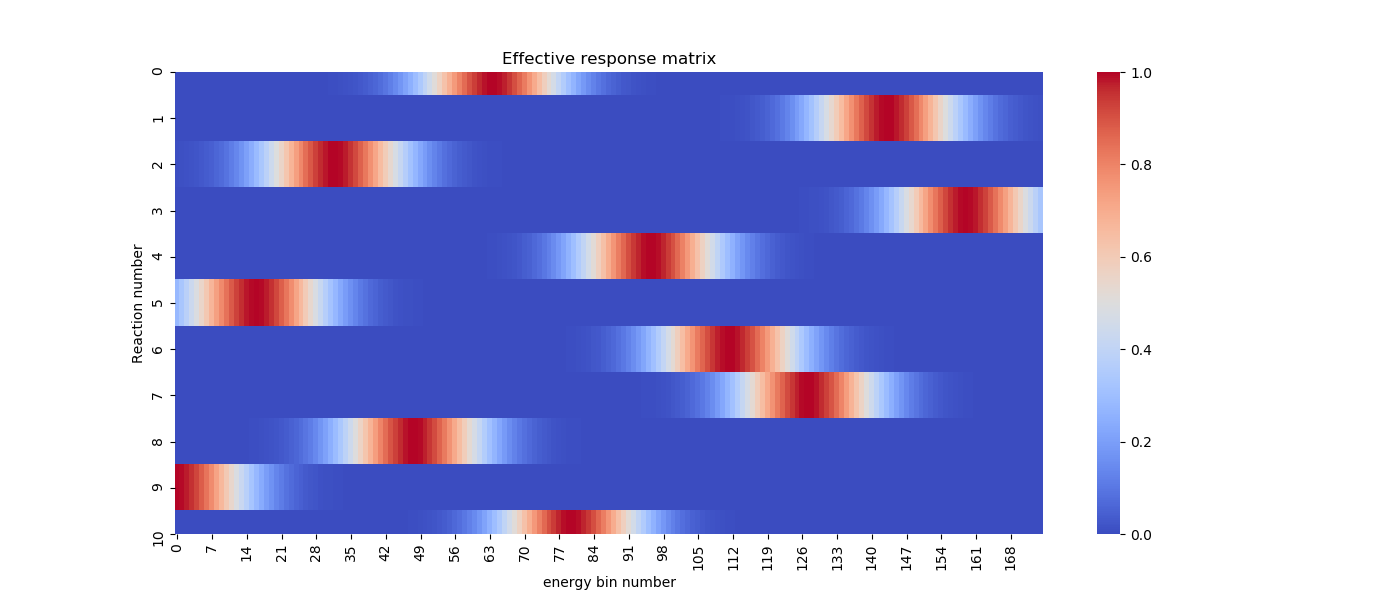
\includegraphics[width=1\textwidth]{EffectiveResponseMatrix.png} %Stupid latex doesn't allow two dots in the filename.
\caption{An example effective response matrix plotted as using \texttt{seaborn.heatmap(R)}, from a distribution of Gaussian peaks. It is very difficult to construct such a well covered matrix in real life.} \label{Example effective response matrix}
\end{figure}

% For reasons which will be justified later in this text, 
The larger the value of $\sum\limits_k R'_{ki}$ is, the more intensely the system samples that part of the spectrum.

\subsection{Criteria for a good effective response matrix}\label{criteria}
A good response matrix should not leave large parts of the spectrum unsampled (i.e. have a ``cool" column).

Also, if one wishes to compare the difference in fluxes of two regions, then one must sample these parts of the spectrum using two different reaction. For example, if one wishes to know how many neutrons gets upscattered/blue-shifted to above bin 169, relative to how many neutrons are present below 169, then there must be at least two separate reactions, e.g. $k=1$ and $k=2$, such that $(R'_{1i}-R'_{2i})$ must experience a drastic change in value as $i$ increases from $i<169$ to $i>169$.

\section{Final number of daughter nuclide and its associated error}
The final number of daughter nuclide for each neutron induced reaction k $= (N_0)_k$.

Given $\lambda_k$ as the decay rate of the daughter nuclide for reaction $k$, \\
$\gamma_k$ as the branching ratio of these decays which leads to a detectable gamma,\\
$\Omega$ as the geometric efficiency of the detection set-up, which, for the current intends and purpose, can be kept as 0.5. \\
$\epsilon_k$ as the photopeak efficiency of the detector at the energy of the gamma that the daughter nuclide emits,

\begin{align}
    (C_0)_k &= \epsilon_{k} \Omega \gamma_{k} \lambda_k (N_0)_k\\
    (N_0)_k &= \frac{1}{\lambda_k \Omega} \frac{1}{\epsilon_{k} \gamma_{k}} (C_0)_k\\
    \sigma(N_0)_k &= \frac{1}{\lambda_k \Omega} \frac{1}{\epsilon_{k} \gamma_{k}} \sigma(C_0)_k\\
    \sigma(N_0)_k &= \frac{1}{\lambda_k \Omega} \frac{1}{\epsilon_{k} \gamma_{k}} \sqrt{C_0}_k \label{error on final number of nuclide}
\end{align}

Equation \ref{reduced effective matrix} then becomes
\begin{align}
    R_{ki}' = V_k \frac{0.5 (N_d)_k\epsilon_{k}\gamma_{k} \lambda_k }{\sqrt{C_0}_k} \sigma_{ki}
\end{align}
Assuming that there is only one type of gamma radiation emitted from the foil to the detector, we can set the count rate $(C_0)_k$ to as high as we can, i.e. $(C_0)_k \leq$ the paralysis limit of the detector. Note that this may also be dependent on the energy of the gamma.

This equation has the dimensionality of (area) on both sides.

\section{Manual foil selection}
The product of $V_k \Omega_k$ acts to scale the reaction rate associated with each foil up or down. Equivalently we can simply fix $\Omega=\frac{1}{2}$ (i.e. place foil directly onto detector when measuring) and only change the volume.

\begin{itemize}
    \item Reaction with the same parent foil will be scaled up/down together (when the daughter's decay is not accounted for) if one were to increase/decrease its volume. This means these rows, as seen in figure \ref{Example effective response matrix}, will get hotter/cooler together. Meanwhile, the ratio between them remains fixed.
    \item Despite what was said in section \ref{Response Matrix For Effectiveness Comparison}, a fast decaying element \emph{can} be used, but in that case the value obtained from equation \ref{reduced effective matrix} will be higher than the true effectiveness (equation \ref{condensed effective matrix}).
    \item There is no harm in adding more reactions to the system (assuming self-shielding is not an issue). However, if space is limited, then one may consider replacing a parent foil that only leads to cool rows on the heatmap with other foils.
    % \item An even distribution of sampling ``duty" across different reaction rates is advised, as as suggested in section \ref{criteria}. 
    \item Sharp changes in \emph{difference} between effective response rates over an area increases the energy resolution of the system over that area, as stated in \ref{criteria}.
    \begin{itemize}
        \item For example, a system consisting of only two threshold reactions with nearly the same profiles (sharp increase, and then plateau), but are off-set from each other by 0.5 MeV, then this system will be able to pick out any variations within that region easily, but are insensitive to regions around them.
    \end{itemize}
    % An effective response matrix containing one a narrow peak in one row and a wide peak in a different row, covering different parts of the spectrum indicate the system has poorer energy resolution over the area covered by the wide peak, but better 
     % See the comparison of \ref{variable peak width}. 
\end{itemize}

\section{Assumption}
The FoilSelector currently does not take into account self-shielding effects, i.e. it assumes that the neutron flux $\phi$ is spatially independent, i.e. $\phi(E,V) = \phi(E)$. 
So that the reaction rate per parent nuclide $Z_k$ is linearly proportional to the average flux and is spatially independent,
\begin{align}
     (N_\infty)_k &= \Delta t \iiiint \sigma_{k}(E) \phi(E,\ve{V}) dE d\ve{V} \\
     (N_\infty)_k &= \Delta t \iiiint \sigma_{k}(E) \phi(E) dE d\ve{V} \\
     (N_\infty)_k &= \Delta t V_k \int \sigma{k}(E) \phi(E) dE \\
     (N_\infty)_k &= \Delta t V_k Z_k \label{scale up daughter per parent per second nuclide to total daughter}
\end{align}
Otherwise, if self-shielding is properly accounted for, \ref{scale up daughter per parent per second nuclide to total daughter} is no longer a spatially independent equation.
% Note that \sigma(\phi_sol) can actually be a covariance matrix instead.
% \bibliographystyle{plain}
% \bibliography{FACTIUNN}


\begin{appendices}
\section{glossary of terminology}
\begin{longtable}{rl}
    $\Delta t$&Time correction factor \\
    $N_\infty$&Number of daughter nuclide generated "per second" initially\\
    $N_\infty$&Number of daughter nuclide generated "per second" after decay
    %Actually I'll need to rewrite this to avoid this N having a dimension of per time problem.
\end{longtable}
\end{appendices}
%`
\end{document}